\documentclass[border=0.2cm]{standalone}
\usepackage{tikz}
\usetikzlibrary{calc}
\begin{document}


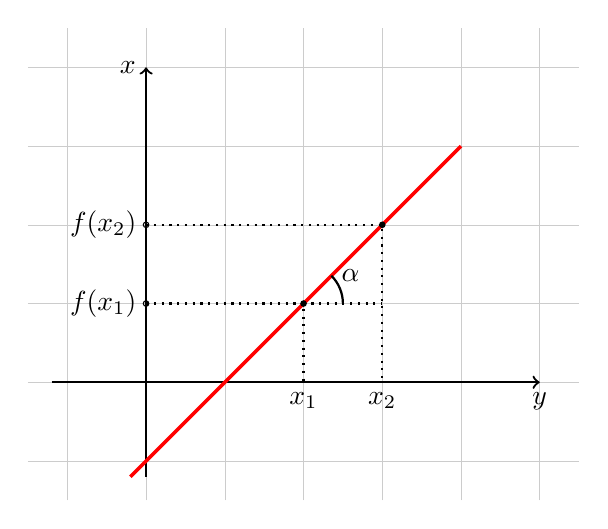
\begin{tikzpicture}
  \draw[help lines,black!20] (-3.5,-2.5) grid (3.5,3.5);
  \draw[thick,->] (-3.2,-1) -- (3,-1) node[below] {$y$};
  \draw[thick,->] (-2,-2.2) -- (-2,3) node[left] {$x$};
  \draw (-2,0) circle (1pt) node[left] {$f(x_1)$};
  \draw (-2,1) circle (1pt) node[left] {$f(x_2)$};

  \draw[line width=1.3pt,red] (-2.2,-2.2) -- (2,2);
  \draw[thick, dotted] (-2,0) -- +(2,0) -- (0,-1) node[below] {$x_1$};

  \draw[thick, dotted] (-2,1) -- +(3,0) -- (1,-1) node[below] {$x_2$};

  \draw[thick, dotted] (0,0) -- (1,0);
  \draw[thick] (.5,0) arc (0:45:0.5) node[right] {$\alpha$};
  
  \fill (1,1) circle (1.2pt);
  \fill (0,0) circle (1.2pt);
  
\end{tikzpicture}



\end{document}